\section{Plasmon}
\label{sec:TheoPlas}

Before delving into nanoplasmonics, this section will provide an introduction to the concept of a plasmon
and elaborate important aspects relevant to this laboratory practice.

A plasmon is a quasiparticle such as a phonon. In contrast to a phonon, the particle is not a vibration of 
the lattice but a collective oscillation of the electrons in response to an interaction of a electromagnetic field, such as light. 
Plasmonics finds applications in fields such as nanophotonic devices, sensing, imaging, optoelectronics, data storage, energy harvesting, and photothermal therapy, enabling advancements in compact photonics, sensitive sensing, high-resolution imaging, efficient solar cells, and targeted cancer treatment.

\subsection*{Bulk plasmons}

Graphically, the plasmon is a motion of electrons, bound to a lattice of positively charged atomic nucleus. When an electric field pushes the 
electrons aside they start wobbling around the nuclei with the plasma frequency $\omega_P$ till the oscillation is dampened. 
These collective oscillations of charge are known as plasmons, specifically referred to as bulk plasmons to differentiate them from surface plasmons discussed later. Since bulk plasmons are longitudinal waves, they are unable to interact with transverse electromagnetic fields and therefore cannot be excited or scattered directly by direct irradiation.

\subsection{Particle plasmons}

Particle plasmon can be seen are a special case of plasmons which are confined in three dimensions. This 
confinement in the nano scale introduces interesting effects as it links the macroscopic properties of the 
material to the quantum mechanical effects reoccurring at the nano scale. In the following we are going to 
investigate this complex effect for nanorods. 

\begin{figure}[ht]
    \centering
    \begin{subfigure}{0.48\linewidth}
      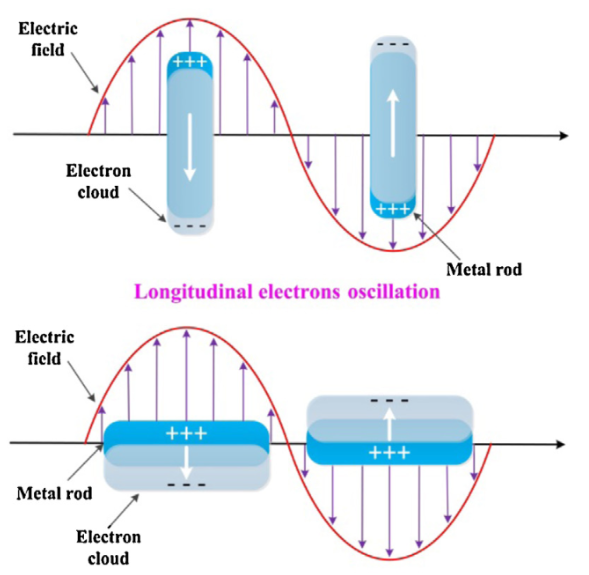
\includegraphics[width=\linewidth]{Bilder/Theory/Nanorod.png}
      \caption{}
      \label{fig:Nanorod}
    \end{subfigure}
    \hfill
    \begin{subfigure}{0.48\linewidth}
      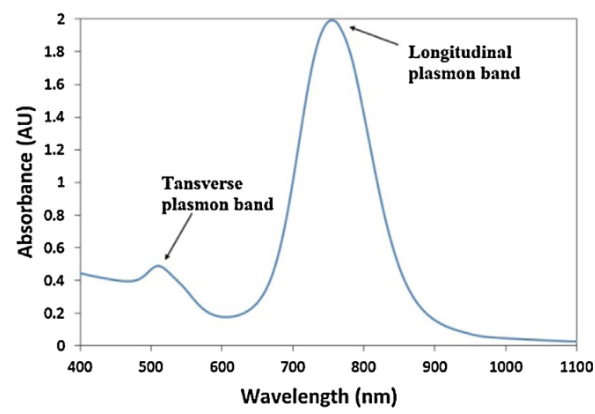
\includegraphics[width=\linewidth]{Bilder/Theory/SpectrumNanorod.png}
      \caption{}
      \label{fig:SpecNanorod}
    \end{subfigure}
    \caption{In (a) a schematic illustration presents the shape of the nanorods. The spectrum in (b) shows the light scattered on the nanorods and detected with dark-field microscopy. From \cite{LehrstuhlExperimentalphysikIII.2023}}
    \label{fig:nanoplasmonics}
\end{figure}

% Nanorods do have two length scales. Therefore the plasmons are confined in 2 dimensions in a different manner. The confinement can be thougth of as 
% as a box as in qumantummechanics. Discrete energy levels reaper. 
% These can scatter. 
% These scattering levels can be observed in Figure (ref).
Nanorods have a double-length scale property, leading to clear confinement of plasmons in two dimensions. This confinement can be envisioned as a quantum mechanical "box," resembling the concept of discrete energy levels. As a result, these confined plasmons give rise to scattering phenomena on these distinct energy levels. Figure \ref{fig:nanoplasmonics} provides data showing the scattering on those levels. As expected, two peaks appear, which correspond to the two ground levels of the two "boxes", one for longitudinal ond one for transversal waves.
This concept allows the experimentalist to access information about length scale way beyond the diffraction limit of optical microscopy.

This box can also be conceptualized as a one dimensional resonator for surface plasmons.
The longitudinal mode of a resonator can be understood as a Fabry-Perot mode. These surface plasmons propagate along the surface of the rod and get reflected at its ends, and thus form standing waves. For the wavelength of the m-th resonance of a perfect resonator with length L, the following relation holds:

\begin{equation}
    \lambda\cdot m = n_{\mathrm{eff}}\cdot 2L(m),
\end{equation}

where $n_{\mathrm{eff}}$ represents the effective refractive index of the plasmon.

Taking this conceptualization, it is to be expected as can be shown in data in (ref) that 

\begin{figure}
    \centering
    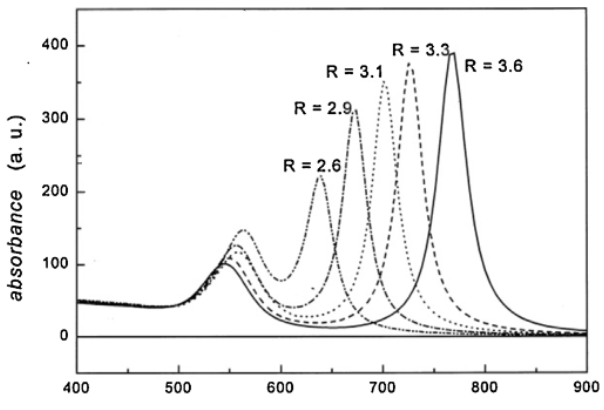
\includegraphics[width = 12cm]{Bilder/Theory/NanorodResonator.png}
    \caption{Absorption spectra of nanorods with different lengths. The aspect ratio R is defined as the ratio between the long and the short side of the rod. As the length of the rod increases, the longitudinal resonance shifts to longer wavelengths. Image from \cite{Link.1999}}
    \label{fig:NanorodResonator}
\end{figure}

In a nanorod, the field of the resonator extends beyond the boundaries of the particle. This results in a slightly elongated resonator, with an extension $\Delta L$ and a resonance wavelength of
\begin{equation}
    \lambda\cdot m = n_{\mathrm{eff}}\cdot 2(L(m)+\Delta L).
\end{equation}

